\section{要求仕様}
本プロジェクトでは、RoboCup 2023で開発したロボットであるHappy Eduを使用する。Fig 1に
ロボットの全体図を示す。Happy Eduのロボット台車は、ROBOTISのTurtleBot3 Big Wheelであり、
ロボット台車の前方に2D-LiDARを搭載している。2D-LiDARは、北表電気株式会社のUTM30-LXを使用
している。制御PCは、NVIDIA GeForce RTX 4070 8GB を搭載しているノートPCを選定した。\\ \indent
以上の構成で以下の要求仕様を設定する。\\
(1) 2D-LiDARのデータで人追従ができる \\
(2) 雑多な状態の空間でも人追従ができる \\
(3) 0.5[m/s]以下の歩行速度で追従する \\

\section{システム構成}
\begin{figure*}[h]
    \begin{center}
    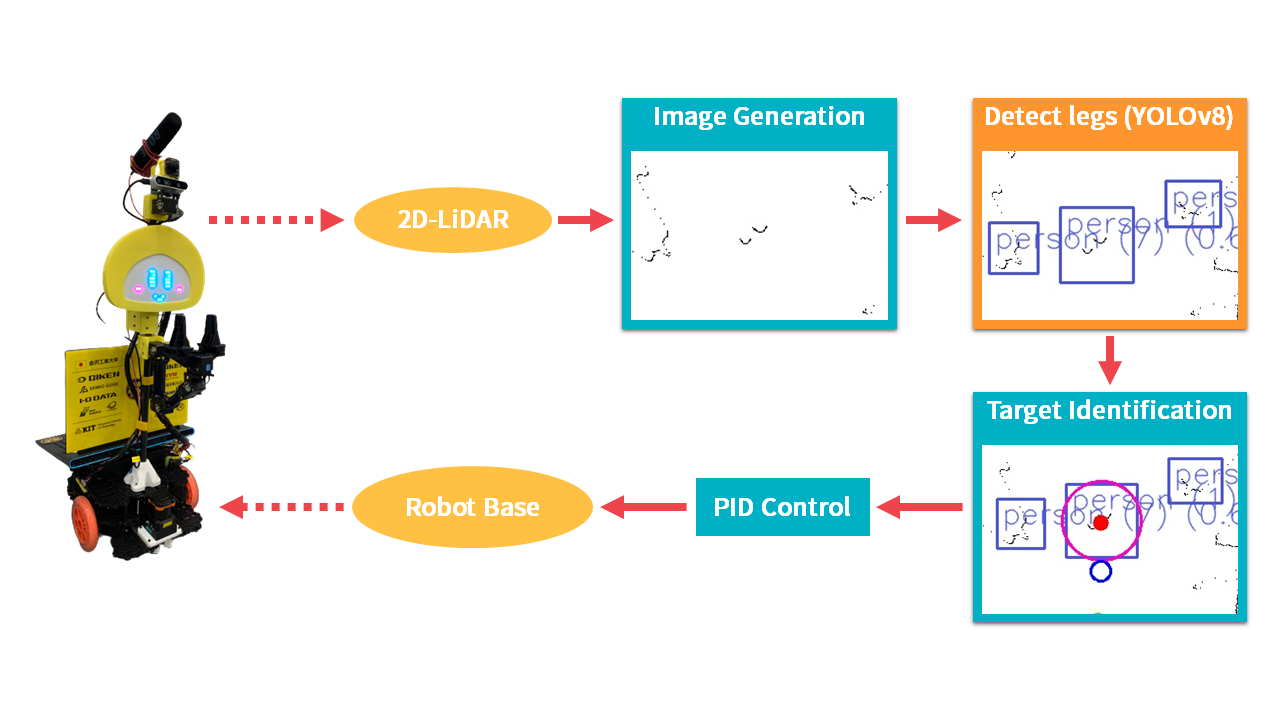
\includegraphics[height=50mm,clip]{figure/システム構成図.png}
    \caption{System configuration chart}
    \label{System configuration chart}
    \end{center}
  \end{figure*}

\section{データセットの作成}
2D-LiDARのデータを俯瞰画像へ変換し、データセットを作成する。
2D-LiDAR のデータは、ロボットが静止した状態で前方に人が2人ランダムに歩行する状態で、
ROS2のBag機能で/scanトピックを保存した。ROS2 Bagのデータを元に12032枚の画像データを生成し、
人の脚部をpersonクラスとしてアノテーションを行った。Fig2にデータセットの例を示す。
また、データセットには、画像の回転処理、モザイク処理、2枚の画像を合成し、新しく1枚の画像を
生成するMix Up処理をすることでデータ拡張を行った。

\section{YOLOv8による学習}
学習では、NVIDIA GeForce RTX 4090 16GBを搭載しているPCを使用し、バッチサイズは12、エポック数
は500で学習を行った。過学習を防ぐため、100エポック以降でEarly Stoppingを設定した。
使用するモデルは、ロボットに搭載する制御PCの処理能力が高いため、YOLOv8で最もパラメータ数の多い
YOLOv8xを用いた。

\section{ロボット台車の制御}
YOLOv8による物体検出での推論結果から目標座標を生成し、ロボットから目標座標までの角度の偏差と
距離の偏差を収束させるためPD制御を実装した。 \\ \indent
時刻$t$での、ロボットの座標から目標座標までの角度の偏差を$\theta(t)$とし、ロボット台車の
エンコーダから取得できる旋回速度$\omega(t)$とすると、ロボット台車の制御量である旋回速度
$u(t)$は以下のようになる。
\begin{equation}
u(t) = K_P \cdot \theta(t) + K_D \cdot \left\{ \frac{d}{dt} \theta(t) - \omega(t) \right\}
\end{equation}
$K_P$、$K_D$は調整パラメータである。(3.1)式の第1項は、ロボットの座標から目標座標までの角度の偏差を
比例制御している。第2項は、実機での制御を考慮し、不足しているまたは過多な制御量を
微分制御により調整している。

\subsection{式の貼り方}
\begin{equation}
HorizontalAngle = (p_x - \frac{W}{2}) \cdot \frac{HFOV}{W}
\end{equation}
\begin{equation}
VerticalAngle = (p_y - \frac{H}{2}) \cdot \frac{VFOV}{H}
\end{equation}
\begin{equation}
x = depth \cdot tan(HorizontalAngel)
\end{equation}
\begin{equation}
y = depth \cdot tan(VerticalAngel)
\end{equation}
where $p_x$ and $p_y$ are the pixels at the center of gravity of the segmentation area. $W$ and $H$ are the image sizes of Realsense D435, and $HFOV$ and $VFOV$ are the angles of view of Realsense D435.
